\chapter{Testing emergence for a small community}
\label{ch:extension}

In the previous chapter we addressed some \textit{ad hoc} design decisions made by \citet{deBoer2000}.
In this chapter we present another extension on the original model by \citet{deBoer2000}.
Instead of using random selection for initiator and imitator pairs, we use a small-community-like network.
This network is based on 5 main groups of agents, each with different influence on each other.
The network can behave both vertical as horizontal, i.e. generational or not.
This extension is a demonstration on how the provided code can be used to easily configure new experiments.


%------------------------------------

\section{Small-community-like network}
\label{sec:network_idea}

\begin{figure}[H]
    \centering
    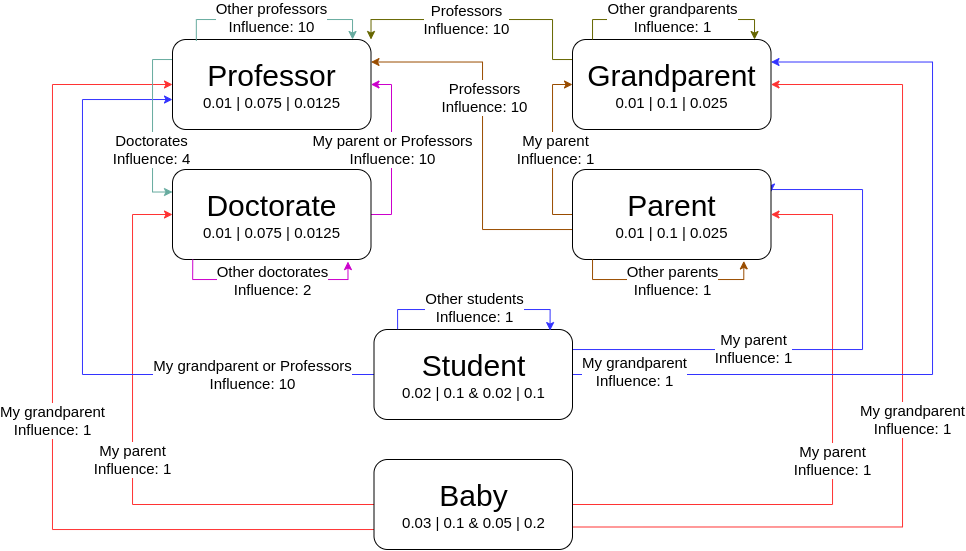
\includegraphics[width=\linewidth]{images/extension/network.png}
    \captionsetup{width=\linewidth}
    \captionsetup{justification=centering}
    \caption{Properties of small community network used.\\Arrows indicate an influential role for the agent accompanied by its weight.\\Notation underneath role: new sound probability $|$ ambient noise $|$ phoneme step size.}
    \label{fig:network}
\end{figure}